\chapter{Background} \label{chap:background}

\section{Inception of Fog Computing}
The inception of Fog Computing comes with the paper published by Bonomi et al. In that paper they discuss a relatively new computing paradigm based on the platform of the Internet of Things. In this paradigm, an extra layer is inserted between the cloud level and end devices level while this layer is not that close to these devices like Edge Computing units but reside a bit more far away in a more centralised way \cite{roman2018mobile}.


\section{Charactistics of Fog Computing}
Bonomi et al. emphasise that Fog Computing is not a substitute for Cloud Computing but an extension. They coined this concept based on the fact that the increasing demand for computing based on automatically created data within IoT networks. The following characteristics can be regarded as the initial motivation of Fog Computing \cite{bonomi2012fog}:
\begin{itemize}
    \item Low latency and location awareness
    \item Wide-spread geographical distribution
    \item Mobility
    \item Vast number of nodes
    \item Predominant role of wireless access
    \item Strong presence of streaming and real-time applications
    \item Heterogeneity
\end{itemize}

The figure \ref{fig:the_internet_of_thing_architecture_and_fog_computing} illustrates the relationship among Cloud Nodes, Fog Nodes and End Devices.

\begin{figure}
    \centering
    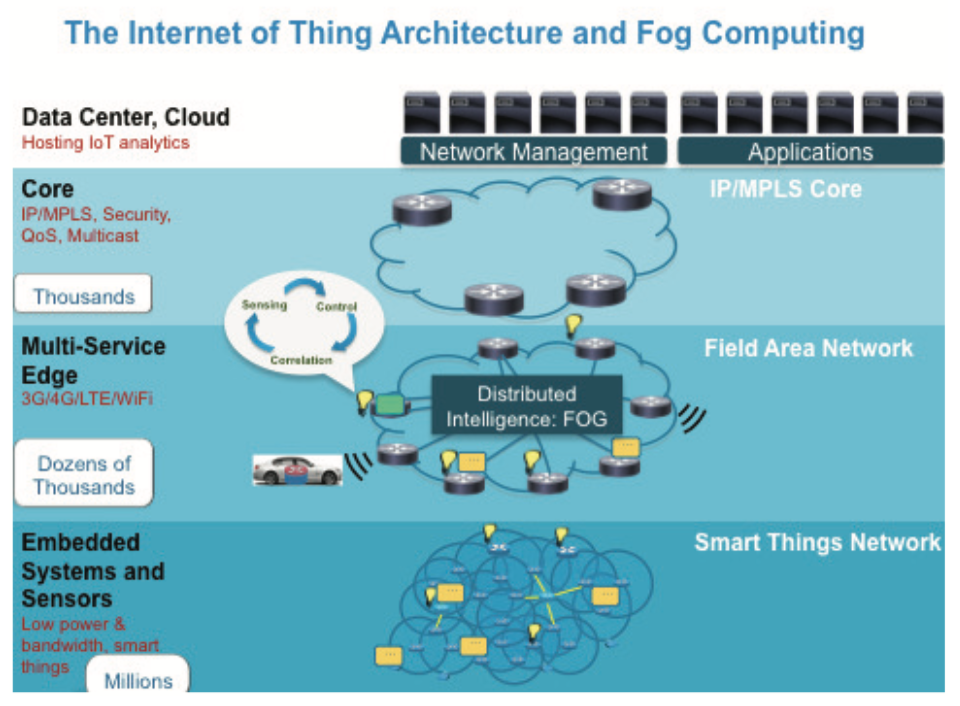
\includegraphics[width=\textwidth]{images/the_internet_of_thing_architecture_and_fog_computing.png}
    \caption{The Internet of Thing Architecture and Fog Computing}
    \label{fig:the_internet_of_thing_architecture_and_fog_computing}
\end{figure}

\section{Scenarios of interest}

\subsection{Connected Vehicle}
Bonomi et al.illustrate a smart traffic light system may become a suitable case applying the Fog Computing. They depict that cars are connected through local network receiving traffic support service, The connection can be via Wi-Fi, 3G, LTE, roadside units and light. In this case, there is a demand that traffic data is under real-time analysis and offer feedback correspondingly, which leading to the requirements of low latency. The high speed of vehicle intensifies the significance of location awareness as well because the algorithm without overall optimisation may provide better speed performance \cite{bonomi2012fog}.

\subsection{Smart Grid}
Smart grid borrows strength from Fog Computing either. The data generated by grid sensors and devices can get processed at the first tier of the Fog, called machine to machine interaction. The rest of the layers provide the analytic functionality of big data processing. 

\subsection{Wireless Sensor and Actuators Networks}
Wireless Sensors nodes are designed as extremely low-power devices, which may benefit from the shared computing capability via fog nodes. All relevant energy constrained devices are considered as advocates of the similar concept.

\subsection{Smart Building}
Beside three scenarios discussed in the paper written Bonomi et al., Stojmenovic et al. complement two other scenarios. Smart building is one of them.

In the scenario of Smart Building, temperature, humidity and appropriate environment measurements are collected and interact with each other via higher level fog node\cite{stojmenovic2014fog}.

\subsection{Software Defined Network}
With SDN gaining attention, studies based on it expanded to the area of Fog Computing. Stojmenovic et al. explain the Fog Computing can be used in the vehicular network to apply the concept of Software Defined Network since it helps separate control and data communication layers. Furthermore, lack of communication among peers in the vehicular network makes Fog Computing an alternative solution when it comes to high packet loss rate \cite{stojmenovic2014fog}.

\subsection{Augmented Reality}
Yi et al. introduce more realistic scenarios in their paper, and real-time video analytics is one of them \cite{yi2015survey}. They consider the popularity of Augmented Reality products such as Google Glass and Microsoft HoloLens that demand high computation power. AR applications notoriously rely on the processing capability of the hardware. Multiple sources of media are going to combine and calculated simultaneously. What's more, even a bit of latency can be sensed by users and eventually impact the outcome. On the other side, intensive computing tasks consume enormous energy, make the mobility of AR hardware unavailable. 

Fog Computing can be plugged to this case. Since we do not push the computing nodes far away from the data, the latency can be ensured. Meanwhile, it saves the power of the devices because these power-consuming tasks are diverted to external hardware and only basic network I/O is contained.

\subsection{Content Delivery and Caching}
Zhu et al. contribute to another scenario of Fog Computing. In their paper, Fog Computing nodes are used as Content Delivery Network nodes. They believe that most of the time wasted in the front-end rendering and execution can be saved if the cache gets optimised and static resources are better compressed. Their concept of Fog Computing is a higher level of Edge Computing. In other words, Fog Computing nodes are more centralised and offer the bridge between cloud and end users. In the scenario, the end users are equipped with computing power to some degree and are not as power sensitive as nodes in wireless networks. As a result, higher level Fog Computing nodes play the role of distributed tasks of Cloud Computing. They help preprocess web objects, page components and minimise traffic.

\subsection{Mobile Big Data Analytic}
The same authors also mention the significance of Fog Computing in the scenario of big data processing. Consider the high demand of Cloud Computing as the resource of big data analysis; relevant tasks pop up dramatically. Sometimes, the Cloud Computing nodes are far away from end users, and low latency top the requirement, Fog Computing nodes become a decent alternative. In this use case, Fog Computing strengthens their feature of elasticity and scalability just like the Could counterpart.